\subsection{Substituierbarkeit}
\label{sec:Kap-9.2.2}

Wir haben das Konzept der Generalisierung (und umgekehrt Spezialisierung) von Klassen im Zusammenhang mit der Realweltmodellierung in Kapitel~4 %todo Kapitel~\ref{sec:Kap-4}
eingeführt. Zur Erinnerung: eine generelle Klasse beschreibt Gemeinsamkeiten von spezielleren Klassen. Jedes Objekt einer spezielleren Klasse ist auch ein Objekt der generelleren Klasse, hat alle dort vergebenen Attribute, kann aber zusätzliche Attribute haben, die nur in der Spezialisierung vorkommen.

Wenn wir uns nun Generalisierung und Spezialisierung im Kontext der Implementierung ansehen, spielen neben Attributen auch Operationen eine Rolle. Jede für eine generellere Klasse definierte Operation kann grundsätzlich für alle Objekte dieser Klasse durchgeführt werden, also auch für alle Objekte, die zu einer spezielleren Klasse gehören. Um im Folgenden die fast unlesbaren Begriffe „generellere“ und „speziellere“ zu vermeiden, wollen wir ein abstraktes Beispiel ansehen:

\sttpUMLText{A} und \sttpUMLText{B} seien Klassen mit folgender Beziehung: \sttpUMLText{A} ist Generalisierung von \sttpUMLText{B}, und umgekehrt \sttpUMLText{B} Spezialisierung von \sttpUMLText{A}. Dies bedeutet insbesondere, dass jedes Objekt von \sttpUMLText{B} auch ein Objekt von \sttpUMLText{A} ist. Wir nennen \sttpUMLText{A} auch Oberklasse und \sttpUMLText{B} Unterklasse (s.~Abb.~\ref{fig:oberklasse_unterklasse}).

\vspace{-2mm} %%% für Druck

\begin{figure}[h!]
	\centering
	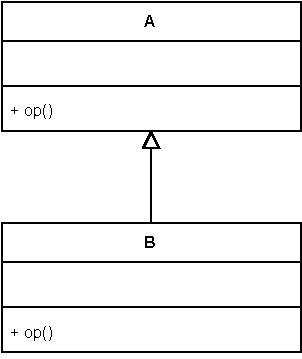
\includegraphics{Bilder/Kapitel-9/oberklasse_unterklasse.pdf}
	\caption{Oberklasse \sttpUMLText{A} und Unterklasse \sttpUMLText{B}}
	\label{fig:oberklasse_unterklasse}
\end{figure}

\pagebreak %%% für Druck

Was gilt nun für Klasseninvarianten der Oberklasse \sttpUMLText{A}? Diese müssen auch in der Unterklasse \sttpUMLText{B} gültig sein. Umgekehrt kann es für \sttpUMLText{B} zusätzliche Invarianten geben, die in \sttpUMLText{A} nicht erfüllt sein müssen bzw. noch nicht einmal formulierbar sein müssen, wenn sie auf Attribute Bezug nehmen, die nur in der Unterklasse vorkommen.

\vspace{1mm} %%% für Druck

Für unsere Dreiecksklasse betrachten wir drei Beispiele:

\begin{enumerate}
	\item Erstens die Klasse der bunten Dreiecke (\sttpUMLText{FarbigesDreieck}). Jedes bunte Dreieck ist natürlich auch ein Dreieck mit Seitenlängen $a$, $b$ und $c$, hat aber ein zusätzliches Attribut \sttpUMLText{Farbe}. 
	\vspace{2mm}
	\begin{center}
		\begin{tikzpicture}[scale=0.7,rotate=12]
			\large
			
			\coordinate (A) at (3,3);
			\coordinate (B) at (0,0);
			\coordinate (C) at (4,0);
			
			\draw (B) -- (C) node[pos=0.5, below right] {$a$};
			\draw (C) -- (A) node[pos=0.5, above right] {$b$};
			\draw (A) -- (B) node[pos=0.5, above left] {$c$};
			
			\fill[FernUni-MI-green-light] (B) -- (C) -- (A) -- cycle;
			\draw[FernUni-MI-green, ultra thick] (B) -- (C) -- (A) -- cycle;
		\end{tikzpicture}
	\end{center}
	\vspace{2mm}
	
	\item Zweitens die Klasse der rechtwinkligen Dreiecke (\sttpUMLText{RechtwinkligesDreieck}). Hier gehen wir davon aus, dass der rechte Winkel zwischen den Seiten $a$ und $c$ besteht.
	\vspace{2mm}
	\begin{center}
		\begin{tikzpicture}[scale=0.7,rotate=-10]
			\large
			
			\coordinate (A) at (0,3);
			\coordinate (B) at (0,0);
			\coordinate (C) at (4,0);
			
			\draw (B) -- (C) node[pos=0.5, below] {$a$};
			\draw (C) -- (A) node[pos=0.5, above right] {$b$};
			\draw (B) -- (A) node[pos=0.5, above left] {$c$};
			
			\draw[very thick] (0.5,0) arc (0:90:0.5);
			\fill (0.2,0.2) circle [radius=0.05];
			
			\draw[FernUni-MI-green, ultra thick] (B) -- (C) -- (A) -- cycle;
		\end{tikzpicture}
	\end{center}
	\vspace{2mm}
	Wir könnten als zusätzliche Attribute die Winkel des Dreiecks aufnehmen. Damit wäre das Dreieck aber überbestimmt, denn es reichen zur Spezifikation des Dreiecks zwei Seiten und ein Winkel oder eine Seite und zwei Winkel (der dritte Winkel folgt aus den beiden anderen ohnehin, denn die Winkelsumme im Dreieck ist stets $180$ Grad). Wir haben aber bereits Attribute für drei Seiten und drücken die Rechtwinkligkeit deshalb über den Satz des Pythagoras aus. Dafür nehmen wir die Invariante $$I_5: b^2 = a^2 + c^2$$ hinzu.

	\item Drittens die Klasse der gleichseitigen Dreiecke (\sttpUMLText{GleichseitigesDreieck}). 
	\vspace{2mm}
	\begin{center}
		\begin{tikzpicture}[scale=0.7,rotate=-15]
			\large
			
			\coordinate (A) at (2,3.46);
			\coordinate (B) at (0,0);
			\coordinate (C) at (4,0);
			
			\draw (B) -- (C) node[pos=0.5, below] {$a$};
			\draw (C) -- (A) node[pos=0.5, above right] {$b$};
			\draw (A) -- (B) node[pos=0.5, above left] {$c$};
			
			\draw[FernUni-MI-green, ultra thick] (B) -- (C) -- (A) -- cycle;
		\end{tikzpicture}
	\end{center}
	\vspace{2mm}
	Für gleichseitige Dreiecke gilt neben $I_1$ die Invariante $I_6: a = b = c$. Es ist leicht zu sehen, dass $I_1$ zusammen mit $I_6$ die Invarianten $I_2$ bis $I_4$ impliziert. 
\end{enumerate}

\pagebreak %%% für Druck

Jede der drei beschriebenen Klassen -- \sttpUMLText{FarbigesDreieck}, \sttpUMLText{RechtwinkligesDreieck} und \sttpUMLText{GleichseitigesDreieck} -- ist mögliche Unterklasse der Klasse \sttpUMLText{Dreieck}. Natürlich kann die Fläche eines bunten Dreiecks, eines rechtwinkligen Dreiecks und eines gleichseitigen Dreiecks ebenfalls mit Herons Formel berechnet werden. Bei bunten Dreiecken gibt es offenbar auch keine bessere Lösung. Die Fläche eines rechtwinkligen Dreiecks dagegen ist viel leichter zu ermitteln, denn es gilt in diesem Spezialfall

$$F = \frac{a \cdot c}{2}.$$

Und auch für gleichseitige Dreiecke gibt es eine Vereinfachung: 

$$ F = \frac{\sqrt{3}}{4} \cdot a^2 .$$

Beides ist wesentlich einfacher zu implementieren als Herons Formel und insbesondere schneller zu berechnen ($\frac{\sqrt{3}}{4}$ ist eine Konstante (0,43301270189…), die Teil des Programmcodes sein kann). 
		
Wenn wir also die Fläche eines rechtwinkligen oder eines gleichseitigen Dreiecks berechnen wollen, können wir Herons Formel nutzen oder auch die einfacheren Formeln, die aber nur eingeschränkt für diese Spezialfälle einsetzbar sind. Entsprechend können wir in den Unterklassen die Implementierung der Operation Flächenberechnung von der Oberklasse erben, oder aber durch effizientere Implementierungen überschreiben, die bei Gültigkeit entsprechender Invarianten dasselbe leisten. Wenn wir Operationsimplementierungen aber überschreiben, müssen wir darauf achten, dass das Liskovsche Substituierbarkeitsprinzip nicht verletzt wird.

\vspace{-2mm} %%% für Druck

\sttpDefinitionskasten{\sttpDefinitionskastenSkalierungsfaktor}{Substituierbarkeitsprinzip}{}{Wenn \sttpUMLText{B} eine Unterklasse einer Klasse \sttpUMLText{A} ist, können Objekte von \sttpUMLText{A} durch Objekte von \sttpUMLText{B} ersetzt werden, ohne dass sich das Verhalten (oder die Korrektheit) ändert.}

\vspace{-5mm} %%% für Druck

\sttpAutorenkasten{Barbara Liskov}{1939}{}{Amerikanische Informatikerin. Promovierte 1968 als erste Frau in den USA in Informatik. Für ihre bedeutenden Leistungen im Design von Programmiersprachen wurde sie mit dem Turing Award ausgezeichnet. Als Professorin lehrte sie am MIT -- Massachusetts Institute of Technology -- Elektrotechnik und Informatik.}{Bilder/Autoren/liskov.jpg}{2010}{Kenneth C. Zirkel, \href{http://creativecommons.org/licenses/by-sa/3.0}{CC BY-SA 3.0}, via \href{https://commons.wikimedia.org/wiki/File:Barbara_Liskov_computer_scientist_2010.jpg}{Wikimedia Commons}}

\pagebreak %%% für Druck

Wenn dies der Fall ist, sprechen wir im Kontext des Entwurfs von \textit{Generalisierung}\marginline{Generalisierung}, ansonsten lediglich von \textit{Vererbung}.

Damit die Objekte der Unterklasse die Objekte ihrer Oberklasse semantiktreu vertreten können, ist es erforderlich, dass die Spezifikation der Unterklasse zur Spezi\-fika\-tion der Oberklasse \textit{konform}\marginline{Konformität} ist. Statt über die Implementierungen selbst argumentieren wir also über ihre Spezifikationen, die indirekt das Verhalten der implementierten Operationen beschreiben.

Wir bezeichnen mit \sttpUMLText{op\textsubscript{A}} bzw. \sttpUMLText{op\textsubscript{B}} eine in den Klassen \sttpUMLText{A} implementierte bzw. in \sttpUMLText{B} überschriebene Operation \sttpUMLText{op()}. Die (Spezifikation der) Operation \sttpUMLText{op\textsubscript{B}} aus \sttpUMLText{B} heißt konform zur (Spezifikation der) in der Klasse \sttpUMLText{A} definierten Operation \sttpUMLText{op\textsubscript{A}}, wenn die folgenden drei \textit{Konformitätsbedingungen} gelten:

\begin{enumerate}
	\item \sttpUMLText{op\textsubscript{B}} und \sttpUMLText{op\textsubscript{A}} 
		\marginline{Konformitäts\-bedingungen}
		haben die gleiche Signatur (d.h., \sttpUMLText{op\textsubscript{B}} überschreibt \sttpUMLText{op\textsubscript{A}}),
	\item Vorbedingung(\sttpUMLText{op\textsubscript{A}}) $\Rightarrow$ Vorbedingung(\sttpUMLText{op\textsubscript{B}}) und
	\item Nachbedingung(\sttpUMLText{op\textsubscript{B}}) $\Rightarrow$ Nachbedingung(\sttpUMLText{op\textsubscript{A}}).
\end{enumerate}

Die Übereinstimmung der Signatur ist eine generelle Voraussetzung dafür, dass die Implementierung \sttpUMLText{op\textsubscript{B}} die Implementierung \sttpUMLText{op\textsubscript{A}} überschreiben kann. Die gegenläufigen Implikationen\footnote{bitte machen Sie sich ggf. unbedingt mit Implikationen vertraut!} zwischen den Vor- und Nachbedingungen sind leicht zu begründen: Wir betrachten einen Zustand, in dem die Vorbedingungen von \sttpUMLText{op\textsubscript{A}} gelten. Dann wird das relevante Verhalten von \sttpUMLText{op\textsubscript{A}} durch seine Nachbedingungen ausgedrückt, die insbesondere das Ergebnis der Ausführung beschreiben. Jede gleich\-wertige Implementierung muss also gewährleisten, dass nach ihrer Ausführung ebenfalls die Nachbedingungen von \sttpUMLText{op\textsubscript{A}} gelten. In dem betrachteten Zustand gelten wegen der ersten Implikation mit den Vorbedingungen von \sttpUMLText{op\textsubscript{A}} auch die Vorbedingungen von \sttpUMLText{op\textsubscript{B}}. Dessen Implementierung stellt sicher, dass im Zustand nach Ausführung von \sttpUMLText{op\textsubscript{B}} die Nachbedingungen \sttpUMLText{op\textsubscript{B}} gelten. Die zweite Implikation besagt nun gerade, dass in diesem Zustand die Nachbedingungen von \sttpUMLText{op\textsubscript{A}} ebenfalls gelten. 

Abb.~\ref{fig:konformitaet} stellt den Sachverhalt graphisch dar.

\begin{figure}[h!]
	\centering
	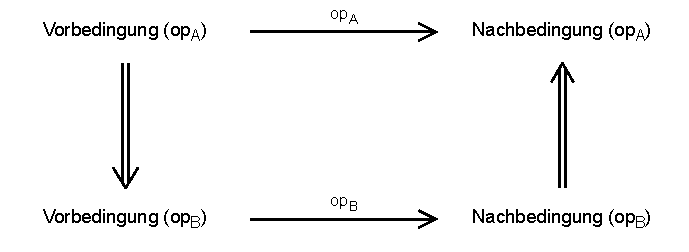
\includegraphics{Bilder/Kapitel-9/konformitaet.pdf}
	\vspace{\baselineskip} %%% für Druck
	\caption{Konformität der Unterklasse \sttpUMLText{B} zur Oberklasse \sttpUMLText{A}}
	\label{fig:konformitaet}
\end{figure}

\pagebreak %%% für Druck

\sttpUMLText{INV\textsubscript{A}} bzw. \sttpUMLText{INV\textsubscript{B}} bezeichnen im Weiteren die Invarianten der Klassen \sttpUMLText{A} bzw. \sttpUMLText{B}. Sind alle überschriebenen Operationen in \sttpUMLText{B} konform zu den entsprechenden Operationen in \sttpUMLText{A} und gilt darüber hinaus \sttpUMLText{INV\textsubscript{B}} $\Rightarrow$ \sttpUMLText{INV\textsubscript{A}}, so heißt die (Spezifikation der) Unterklasse \sttpUMLText{B} \textit{konform} zur (Spezifikation der) Oberklasse~\sttpUMLText{A}.

Die Definition der Konformität präzisiert das Prinzip der Substituierbarkeit:\marginline{Substituier\-barkeit} Ist die Klasse \sttpUMLText{B} konform zur Klasse \sttpUMLText{A}, dann können Instanzen der Klasse \sttpUMLText{A} durch Instanzen der Klasse \sttpUMLText{B} ersetzt werden.

Damit lässt sich jetzt auch die Definition der Generalisierung präzisieren:

\sttpDefinitionskasten{\sttpDefinitionskastenSkalierungsfaktor}{Generalisierung}{}{Eine Ober-Unterklassenbeziehung bezeichnen wir als Generalisierung, wenn die Unterklasse konform zur Oberklasse ist.}

Für die Spezifikation von in der Unterklasse zusätzlich definierten Operationen \mbox{besteht} keine Einschränkung.

Ist die Unterklasse zu ihrer Oberklasse nicht konform, \marginline{Generalisierung vs. Vererbung} sprechen wir anstelle von Generalisierung von Vererbung. Im Kontext von Programmiersprachen wird meistens der Begriff Vererbung verwendet, da weder heute verfügbare Compiler- noch Laufzeitsysteme die Konformität einer Vererbungsbeziehung überprüfen.

Generalisierung im Sinne der Konformität bietet gegenüber der allgemeineren Vererbung erhebliche Vorteile. So lässt sich beispielsweise das Konzept des Vertragsentwurfs bei vertragsgemäßer Programmierung, das die Rechte und Pflichten von Dienstnutzern und Dienstleistern klar regelt, direkt auf Unterklassen der Dienst\-leister übertragen, sofern diese konform zu ihren Oberklassen sind.

Ein weiterer Vorteil ergibt sich für das Testen. Ist (die Spezifikation) einer Klasse \sttpUMLText{B} konform zu (der Spezifikation) einer Klasse \sttpUMLText{A} und sind die Implementierungen von \sttpUMLText{A} und \sttpUMLText{B} gegen ihre Spezifikationen erfolgreich getestet oder verifiziert, so brauchen Operationen, die als Parameter Objekte der Klasse \sttpUMLText{A} erwarten, nicht zusätzlich mit Objekten der Klasse \sttpUMLText{B} als Parameter getestet zu werden.

Kehren wir zurück zu unseren Dreieckklassen. Die Unterklasse \sttpUMLText{FarbigesDreieck} unterscheidet sich bezüglich Invarianten von der Oberklasse nicht, und die Opera\-tion zur Flächenberechnung berührt das Attribut Farbe nicht. Hier ist die Konformität also offensichtlich gegeben. Die Unterklasse \sttpUMLText{RechtwinkligesDreieck} hat eine zusätzliche Invariante. Die Gesamtheit ihrer Invarianten impliziert daher die Invarianten der Oberklasse. Für die Unterklasse \sttpUMLText{GleichseitigesDreieck} haben wir bereits gesehen, dass ihre Invarianten die Invarianten der Oberklasse implizieren.

Die Spezifikationen der Operation stimmen überein, und für die Implementierungen gilt, dass das Ergebnis der beiden effizienteren Flächenberechnungen mit dem Ergebnis der Flächenberechnung nach Heros Formel ebenfalls übereinstimmt, ggf. abgesehen von geringen Rundungsabweichungen. 

\pagebreak %%% für Druck

Um die Konformitätsbedingung zu erläutern, betrachten wir den Fall, dass fälschlich für gleichseitige Dreiecke die hier falsche Formel $\frac{a \cdot c}{2} $ zur Anwendung kommt. In diesem Fall ergibt sich eine andere Nachbedingung, die eben nicht mehr den Flächen\-inhalt beschreibt. Diese Nachbedingung impliziert insbesondere nicht die Nachbedingung der Operation in der Oberklasse. Wenn wir also die Operation fehlerhaft überschreiben, dann kann ein Objekt der Oberklasse (dort wird die korrekte Operation aufgerufen) durch ein Objekt der Unterklasse (dort kommt etwas anderes heraus) nicht semantiktreu ersetzt werden.

Wir betrachten nun eine weitere Operation, die die Wahl unserer Unterklassen der Dreiecke begründet. In dieser Operation wird ein Dreieck in der Dimension der Seite $a$ um einen Faktor $k$ gestreckt. Nach der Streckung ist die Länge dieser Seite $k \cdot a$. Was geschieht mit den anderen Seiten? Die auf $a$ senkrecht stehende Höhe $h$ bleibt unverändert. Die in folgender Abbildung dargestellten Abschnitte $p$ und $q$ der Seite $a$ wachsen ebenfalls um den Faktor $k$.

\begin{center}
	\begin{minipage}[c]{.3\linewidth} 
		\begin{tikzpicture}[scale=0.65,rotate=15]
			\large
			
			\coordinate (A) at (3,3.5);
			\coordinate (B) at (0,0);
			\coordinate (C) at (5,0);
			\coordinate (H) at (3,0);
			
			\draw (B) -- (C) node[pos=0.5, below] {$a$};
			\draw (C) -- (A) node[pos=0.5, above right] {$b$};
			\draw (A) -- (B) node[pos=0.5, above left] {$c$};
			\draw (A) -- (H) node[pos=0.5, right] {$h$};
			\draw (B) -- (H) node[pos=0.5, above] {$p$};
			\draw (H) -- (C) node[pos=0.5, above] {$q$};
			
			\draw[FernUni-MI-green] (A) -- (H);
			\draw[FernUni-MI-green, ultra thick] (B) -- (C) -- (A) -- cycle;
		\end{tikzpicture}
	\end{minipage}
	\textcolor{FernUni-MI-green}{\Huge $\leadsto$}~~~~~
	%\hspace{.05\linewidth}% Abstand zwischen den beiden Bildern
	\begin{minipage}[c]{.4\linewidth}
		\begin{tikzpicture}[scale=0.65,rotate=15]
			\large
			
			\coordinate (A) at (4.5,3.5);
			\coordinate (B) at (0,0);
			\coordinate (C) at (7.5,0);
			\coordinate (H) at (4.5,0);
			
			\draw (B) -- (C) node[pos=0.5, below right] {$k \cdot a$};
			\draw (C) -- (A) node[pos=0.5, above right] {$b_k$};
			\draw (A) -- (B) node[pos=0.5, above left] {$c_k$};
			\draw (A) -- (H) node[pos=0.5, right] {$h$};
			\draw (B) -- (H) node[pos=0.5, above] {$k \cdot p$};
			\draw (H) -- (C) node[pos=0.5, above] {$k \cdot q$};
			
			\draw[FernUni-MI-green] (A) -- (H);
			\draw[FernUni-MI-green, ultra thick] (B) -- (C) -- (A) -- cycle;
		\end{tikzpicture}
	\end{minipage}
\end{center}

Während vor der Streckung die Gleichungen 
$$c^2 = p^2 + h^2,$$
$$b^2 = q^2 + h^2$$
gelten, erhalten wir nach der Streckung für die neuen Seiten
$c_k$ und $b_k$ die Gleichungen 
$$ c_k^2 = k^2 \cdot p^2 + h^2,$$ 
$$ b_k^2 = k^2 \cdot q^2 + h^2$$
und die Ergebnisse durch Ziehung der Wurzel. Deutlich wird, dass $b$ und $c$ um einen geringeren Faktor als $k$ gestreckt werden (und im Fall $p=0$ verändert sich $c$ gar nicht).

Nach Anwendung dieser Operation bleibt ein (beliebiges) Dreieck ein (beliebiges) Dreieck und ein farbiges Dreieck bleibt farbig. Bei einem rechtwinkligen Dreieck bleibt der rechte Winkel bestehen, das Resultat erfüllt damit immer noch die Klassen\-invariante. Aus einem gleichseitigen Dreieck wird dagegen ein gleichschenkliges, und das resultierende Objekt gehört gar nicht mehr in diese Unterklasse. $I_6$ ist keine Invariante mehr. In diesem Fall kann daher nicht mehr von Generalisierung gesprochen werden.

Ein weiteres Beispiel, in dem die Verletzung der Konformität nicht mit dem Überschreiben einer Operation der Oberklasse zusammenhängt, kommt aus einem ganz anderen Bereich:

\begin{figure}[h!]
	\centering
	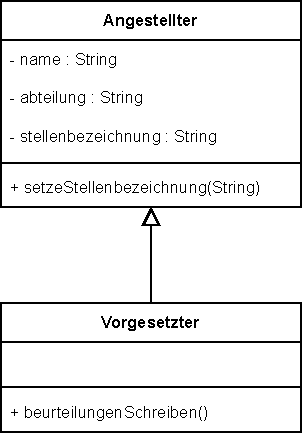
\includegraphics{Bilder/Kapitel-9/angestellter_vorgesetzter.pdf}
	\caption{Vorgesetzte sind spezielle Angestellte}
	\label{fig:angestellter_vorgesetzter.pdf}
\end{figure}

Abbildung~\ref{fig:angestellter_vorgesetzter.pdf} zeigt die Klasse \sttpUMLText{Angestellter}. Diese Klasse enthält das Attribut \sttpUMLText{stellenbezeichnung}, das die Werte "`Programmierer"', "`Administrator"', "`Gruppenleiter"' und "`Abteilungsleiter"' annehmen kann. Die Bedingung, dass andere als diese vier Werte nicht zulässig sind, ist Bestandteil der Klasseninvarianten der Klasse \sttpUMLText{Angestellter}. Die Unterklasse \sttpUMLText{Vorgesetzter} definiert spezielle Angestellte mit Vorgesetztenaufgaben, \zb \sttpUMLText{beurteilungenSchreiben}. Vorgesetzte erben das Attribut \sttpUMLText{stellenbezeichnung} der Klasse \sttpUMLText{Angestellter}, jedoch sind Vorgesetzte immer Gruppenleiter oder Abteilungsleiter, aber niemals Programmierer oder Administrator. Diese Einschränkung ist Bestandteil der Klasseninvariante der Klasse \sttpUMLText{Vorgesetzter}.

Auf den ersten Blick sieht es so aus, als wäre die Klasse \sttpUMLText{Vorgesetzter} konform zur Klasse \sttpUMLText{Angestellter}. Vorgesetzte scheinen Angestellte ersetzen zu können, da keine geerbte Methode überschrieben wird und Vorgesetztenobjekte auch die Invariante für Angestellten-Objekte erfüllen. Probleme gibt es jedoch, wenn ein Vorgesetzter über einen Aufruf der Operation \sttpUMLText{setzeStellenbezeichnung()} \zb zum Programmierer gemacht wird, denn dann verlässt das Vorgesetztenobjekt den zulässigen Zustandsraum für Vorgesetzte und verletzt seine Klasseninvariante. Tatsächlich ist die Klasse \sttpUMLText{Vorgesetzter} zur Klasse \sttpUMLText{Angestellter} nicht konform, da wegen der stärkeren Invariante auch die Vorbedingung von \sttpUMLText{setzeStellenbezeichnung()} stärker sein muss, so dass die Konformitätsbedingung zu Klasseninvarianten für die Operation nicht erfüllt ist.

Die Verletzung der Konformität hat die Konsequenz, dass Vorgesetzte nicht an Stellen verwendet werden können, an denen auf das Attribut \sttpUMLText{stellenbezeichnung} von Angestellten schreibend zugegriffen wird. Bei der vorliegenden Vererbung handelt es sich somit nicht um eine Generalisierung.

Eine konforme Lösung dieses Problems lernen wir gleich im folgenden Abschnitt kennen.